\documentclass[a4paper,11pt,dvipdfmx]{jsarticle}


% 数式
\usepackage{amsmath,amsfonts}
\usepackage{bm}
% 画像
\usepackage[dvipdfmx]{graphicx}
\usepackage{circuitikz}
\usepackage{amsmath,amssymb}
\usepackage{siunitx}
\usepackage{float}
\usepackage{tikz}
\usepackage{askmaps}
\usepackage{multirow}
\usepackage{bigstrut}
\usepackage{rotating}
\usepackage{listings}
% 数式
\usepackage{physics}
\usepackage{mathtools}
% 画像
\usepackage{subcaption}
% 表
\usepackage{makecell}
% その他
\usepackage{url}
\usepackage{ascmac}
\usepackage{cases}
\usepackage{here}
\usepackage{upgreek}

% 画像挿入コマンド
\newcommand{\Figure}[4]{
\begin{figure}[H]
\centering
\includegraphics[width=#1\linewidth]{./images/#2}
\caption{#3}
\label{fig:#4}
\end{figure}
}




\begin{document}

\begin{table}[b]
  \centering
  \begin{tabular}{|c|c|}
    \hline
    報告者     & 22120 222 塚田 勇人 \\
    \hline
    共同実験者 & 22192 234 山本 悠介  \\ & 22060 211 古城 隆人\\
    \hline
    担当者     & 楡井 雅巳 \\
              &  藤澤 義範\\
    &力丸 彩奈\\
    &村田 雅彦\\
    &富岡 雅弘\\
    \hline
    実験年月日 & 2024年10月25日 天気:晴れ 気温:19.1℃ 湿度63\verb#%#\\
    & 2024年11月1日 天気:曇り 気温:15.9℃ 湿度69\verb#%#\\
    & 2024年11月18日 天気:曇り 気温:21.5℃ 湿度55\verb#%#\\
    \hline
    提出期限   & 2024年11月21日 17:00  \\
    \hline
    提出日     & \today              \\
    \hline
  \end{tabular}
\end{table}

\title{セレクタ基板のリバースエンジニアリング}
\author{学籍番号:22120 \\ 組番号:222 \\名前:塚田 勇人}
\date{\today}
\maketitle

\newpage

\section{目的}
電子天秤の作成のために、セレクタ回路のリバースエンジニアリングをし、回路図を作成することを今回の目的とする。

\section{原理}
今回は、セレクタ回路のリバースエンジニアリングを行う。セレクタ回路に関する基本的な知識や使われている電子部品に
ついて説明する。

\subsection{セレクタ回路}
セレクタ回路は複数の入力を持ち、出力する信号を選ぶことが出来る回路である。真理値表を表\ref{tab:selector}に示す。
今回使用するセレクタ基板は入力が$SW1$、$SW0$の2つで、$SW1$、$SW0$の入力によって$A$、$B$、$C$のどれかが出力される。また、
出力は$OUT$と$EN$の2つの信号を持つ。$EN$は有効信号であり、セレクタ回路の先につながる3bitと7セグLEDを
デコードする基板上で、$EN$が$1$の時にのみLEDに出力されるようになっている。そのため$EN$が$0$になるときは$OUT$は何を
出力してもLEDには表示されない。

\begin{table}[H]
\centering
\caption{セレクタ回路の真理値表}
\label{tab:selector}
\begin{tabular}{|cc|cc|}
  \hline
  SW0 & SW1 & OUT & EN\\
  \hline
  OFF & OFF & 0 & 0\\
  ON  & OFF & B & 1\\
  OFF & ON  & C & 1\\
  ON  & ON  & A & 1\\
  \hline
\end{tabular}
\end{table}

\subsection{トグルスイッチ}
トグルスイッチはONとOFFの2つの状態を持つスイッチである。今回使用するトグルスイッチはONの時に$5V$、OFFの時に$GND$を出力する。

\subsection{汎用ロジックIC}
汎用ロジックICは、論理回路を実装するためのICであり、型番によって搭載されている論理ゲートが異なる。
今回使用するICを表\ref{tab:IC}に示す。
\begin{table}[H]
  \centering
  \caption{IC}
  \begin{tabular}{|c|c|}
    \hline
    型番  &  機能  \\
    \hline
    74LS04 & NOTゲート \\
    74LS08 & ANDゲート \\
    74LS32 & ORゲート \\
    \hline
  \end{tabular}
  \label{tab:IC}
\end{table}
ICの内部にはいくつかのトランジスタが内蔵されている。
ここでは例としてNPN型トランジスタの説明をする。NPN型トランジスタは、エミッタ、ベース、コレクタの3つの電極を持つ三端子素子である。
エミッタはGNDに接続、コレクタは出力端子に接続されている。ベースがHighのとき、トランジスタはオンになり、コレクタに電流が流れる。
これをシンク電流という。ベースがLowのとき、トランジスタはオフになり、コレクタに電流が流れずに出力端子側に電流が流れる。
これをソース電流という。

\subsection{セラミックコンデンサ}
セラミックコンデンサは、セラミックを絶縁体として用いたコンデンサである。セラミックコンデンサは、高周波の電流を流す際に
用いられる。

\subsection{バイパスコンデンサ}
バイパスコンデンサは、直流信号を通過させるコンデンサである。

\subsection{動作確認用減算基盤}
今回使用するセレクタ回路の入力をするための基盤を動作確認用減算基盤という。
この基板はセレクタ回路とピンヘッダを介してつながっており、出力は$A= [A_2, A_1, A_0]$、$B = [B_2, B_1, B_0]$、
$C = [C_2, C_1, C_0]$の3つの入力がある。それぞれの出力に対して10進数から2進数にエンコードする回路が入っており、
0から9までの入力をセレクタ回路に渡すことが可能であるが3bitの出力なので、8以上の信号では4bit目が切り捨てされるため0から始まる。
動作確認用減算基盤のピンヘッダのピンアサインを表\ref{tab:pin}に示す。
\begin{table}[H]
  \centering
  \caption{ピンヘッダ}
  \label{tab:pin}
  \begin{tabular}{|c|c|}
    \hline
    $SW1$  & $SW2$  \\
    \hline
    $5V$ & $B2$ \\
    $A2$ & $B1$ \\
    $A1$ & $B0$ \\
    $A0$ & $C2$ \\
    $5V$ & $C1$ \\
    $5V$ & $C0$ \\
    $GND$ & $GND$ \\
    \hline
  \end{tabular}
\end{table}

\subsection{テスター}
テスターは交流・直流どちらでも使用できる電気計測器であり、電圧の測定や電流の測定、電圧を印加して抵抗値を調べるなどのことを
行うことが出来る。今回はテスターを用いることにより、ピンが導通しているかを確認する。

\section{実験方法}
セレクタ回路のリバースエンジニアリングを行うための実験方法について説明する。
まず、回路の実際の動作や簡単なセレクタ回路を理解し、セレクタ回路の回路図を予想する。
次に、マルチテスターを用いて、セレクタ回路の回路を探査し、得られた情報をもとに回路図を作成する。

\subsection{実験に用いた機器}
今回の課題に用いた機器や電子部品について表\ref{tab:equipment}と表\ref{tab:electronicParts}に示す。

\begin{table}[H]
  \caption{実験に用いた機器}
  \centering
  \begin{tabular}{c|c|c}
    \hline
    器具名         & 製造元    & 計器番号    \\
    \hline \hline
    マルチテスター & NISHIZAWA & MODEL 5220  \\
    \hline
    ACアダプタ     & Fksystem  & GF12-US0520 \\
    \hline
  \end{tabular}
  \label{tab:equipment}
\end{table}

\begin{table}[H]
  \caption{実験に用いた電子部品}
  \centering
  \begin{tabular}{c|c|c|c}
    \hline
    部品名               & 諸元          & 個数 & 部品記号 \\
    \hline \hline
    抵抗                 & 10kΩ   & 7    & R1~R2   \\
    \hline
    集積回路(IC)1        & SN74LS04N     & 1    & IC1      \\
    \hline
    集積回路(IC)2        & SN74LS08N     & 3    & IC2~IC4 \\
    \hline
    集積回路(IC)3        & SN74LS32N     & 3    & IC5~IC6 \\
    \hline
    ピンヘッダ           & 2 × 7ピン & 2    & PH1~PH2 \\
    \hline
    トグルスイッチ       & ON-OFF        & 2    & SW0~SW1 \\
    \hline
    セラミックコンデンサ & 0.1µ$F$       & 2    & CA1~CA6 \\
    \hline
  \end{tabular}
  \label{tab:electronicParts}
\end{table}



\subsection{セレクタ回路の動作確認}
まず最初にセレクタ基板にロジックICを挿入し、ピンヘッダを介して動作確認用減算基板、動作確認用デコード基板を接続する。
セレクタ基板の概要図を図\ref{fig:selector}に示す。
$J1$に動作確認用減算基板を接続し、$J2$に動作確認用デコード基板を接続する。
$IC1$から$IC6$に接続する汎用ロジックICを表\ref{tab:IC}に示す。
\Figure{0.8}{kiban.drawio.png}{セレクタ基板の概要図}{selector}
\begin{table}[H]
  \centering
  \caption{IC}
  \begin{tabular}{|c|c|}
    \hline
    部品ID  &  汎用ロジックIC  \\
    \hline
    IC1  &  74LS04  \\
    IC2  &  74LS08  \\
    IC3  &  74LS08  \\
    IC4  &  74LS08  \\
    IC5  &  74LS32  \\
    IC6  &  74LS32  \\
    \hline
  \end{tabular}
\end{table}

\subsection{リバースエンジニアリング}
リバースエンジニアリングを行っていく。このとき導通チェックのためにテスターの端子に電圧を印加させるため、ソケットからICを外して行う。
むやみにテスターを当てていくよりも、最も原始的なセレクタ回路を基にテスターを当てていくことである程度見るピンの数を減らすことが出来る。
最も原始的なセレクタ回路を図\ref{fig:selector}に示す。
\Figure{0.8}{selector.png}{最も原始的なセレクタ回路の基本図}{selector}

\section{実験結果}
セレクタ回路の動作確認とリバースエンジニアリングを行った結果を示す。

\subsection{セレクタ回路の動作確認}
セレクタ回路の動作確認を行った結果を表\ref{tab:selector1}に示す。
3bitしか出力がないため、$(8)_10$以上の数値を入力しても4bit目が切り捨てられるため、$(8)_10$のときは 
\scalebox{0.023}{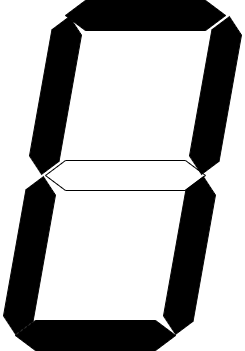
\includegraphics{./images/7segen.drawio.png}} が表示される。
\begin{table}[H]
  \centering
  \caption{セレクタ回路の動作確認}
  \begin{tabular}{|c|c|c|c|c|}
    \hline
    \textrm{$(0)_{10}$} & \textrm{$(1)_{10}$} & \textrm{$(2)_{10}$} & \textrm{$(3)_{10}$} & \textrm{$(4)_{10}$} \\
    \hline
    \begin{minipage}{0.15\columnwidth}
      \centering
      \scalebox{0.15}{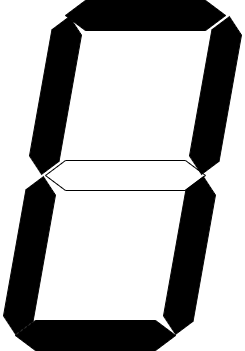
\includegraphics{./images/7seg0.drawio.png}}
    \end{minipage} &
    \begin{minipage}{0.15\columnwidth}
      \centering
      \scalebox{0.15}{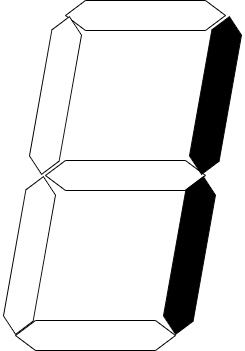
\includegraphics{./images/7seg1.drawio.png}}
    \end{minipage} &
    \begin{minipage}{0.15\columnwidth}
      \centering
      \scalebox{0.15}{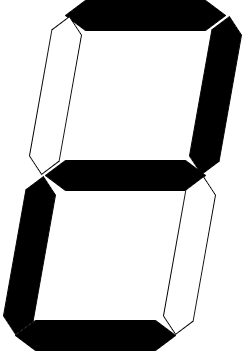
\includegraphics{./images/7seg2.drawio.png}}
    \end{minipage} &
    \begin{minipage}{0.15\columnwidth}
      \centering
      \scalebox{0.15}{
\includegraphics{./images/7seg3.drawio.png}}
    \end{minipage} &
    \begin{minipage}{0.15\columnwidth}
      \centering
      \scalebox{0.15}{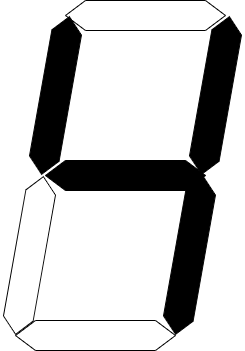
\includegraphics{./images/7seg4.drawio.png}}
    \end{minipage} \\
    \hline
    \textrm{$(5)_{10}$} & \textrm{$(6)_{10}$} & \textrm{$(7)_{10}$} & \textrm{$(8)_{10}$} & \textrm{$(9)_{10}$} \\
    \hline
    \begin{minipage}{0.15\columnwidth}
      \centering
      \scalebox{0.15}{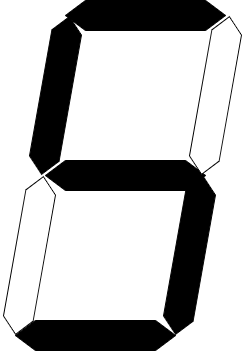
\includegraphics{./images/7seg5.drawio.png}}
    \end{minipage} &
    \begin{minipage}{0.15\columnwidth}
      \centering
      \scalebox{0.15}{
\includegraphics{./images/7seg6.drawio.png}}
    \end{minipage} &
    \begin{minipage}{0.15\columnwidth}
      \centering
      \scalebox{0.15}{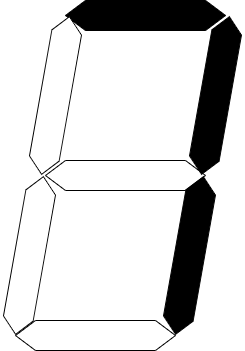
\includegraphics{./images/7seg7.drawio.png}}
    \end{minipage} &
    \begin{minipage}{0.15\columnwidth}
      \centering
      \scalebox{0.15}{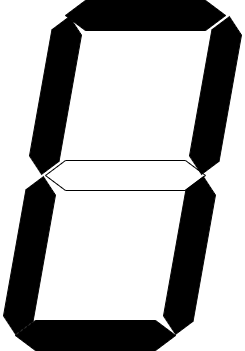
\includegraphics{./images/7segen.drawio.png}}
    \end{minipage} &
    \begin{minipage}{0.15\columnwidth}
      \centering
      \scalebox{0.15}{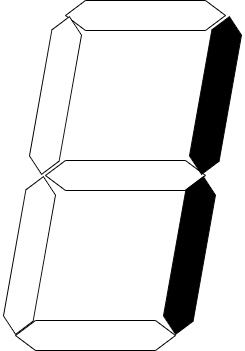
\includegraphics{./images/7seg1.drawio.png}}
    \end{minipage} \\
    \hline
  \end{tabular}
  \label{tab:selector1}
\end{table}

\subsection{リバースエンジニアリング}
リバースエンジニアリングを行って作成した回路図を図\ref{fig:reverse}に示す。
また、作成した回路図を元に真理値表を作成した結果を表\ref{tab:a}に示す。
\begin{table}[H]
  \centering
  \caption{真理値表}
  \begin{tabular}{|cc|cc|}
    \hline
    $SW1$  & $SW2$  &  $OUT$ & $EN$\\
    \hline
    0 & 0 &* & 0 \\
    0 & 1 &$B$ &1 \\
    1 & 0 &$C$ &1 \\
    1 & 1 &$A$ &1 \\
    \hline
  \end{tabular}
  \label{tab:a}
\end{table}

\begin{figure}[H]
  \centering
  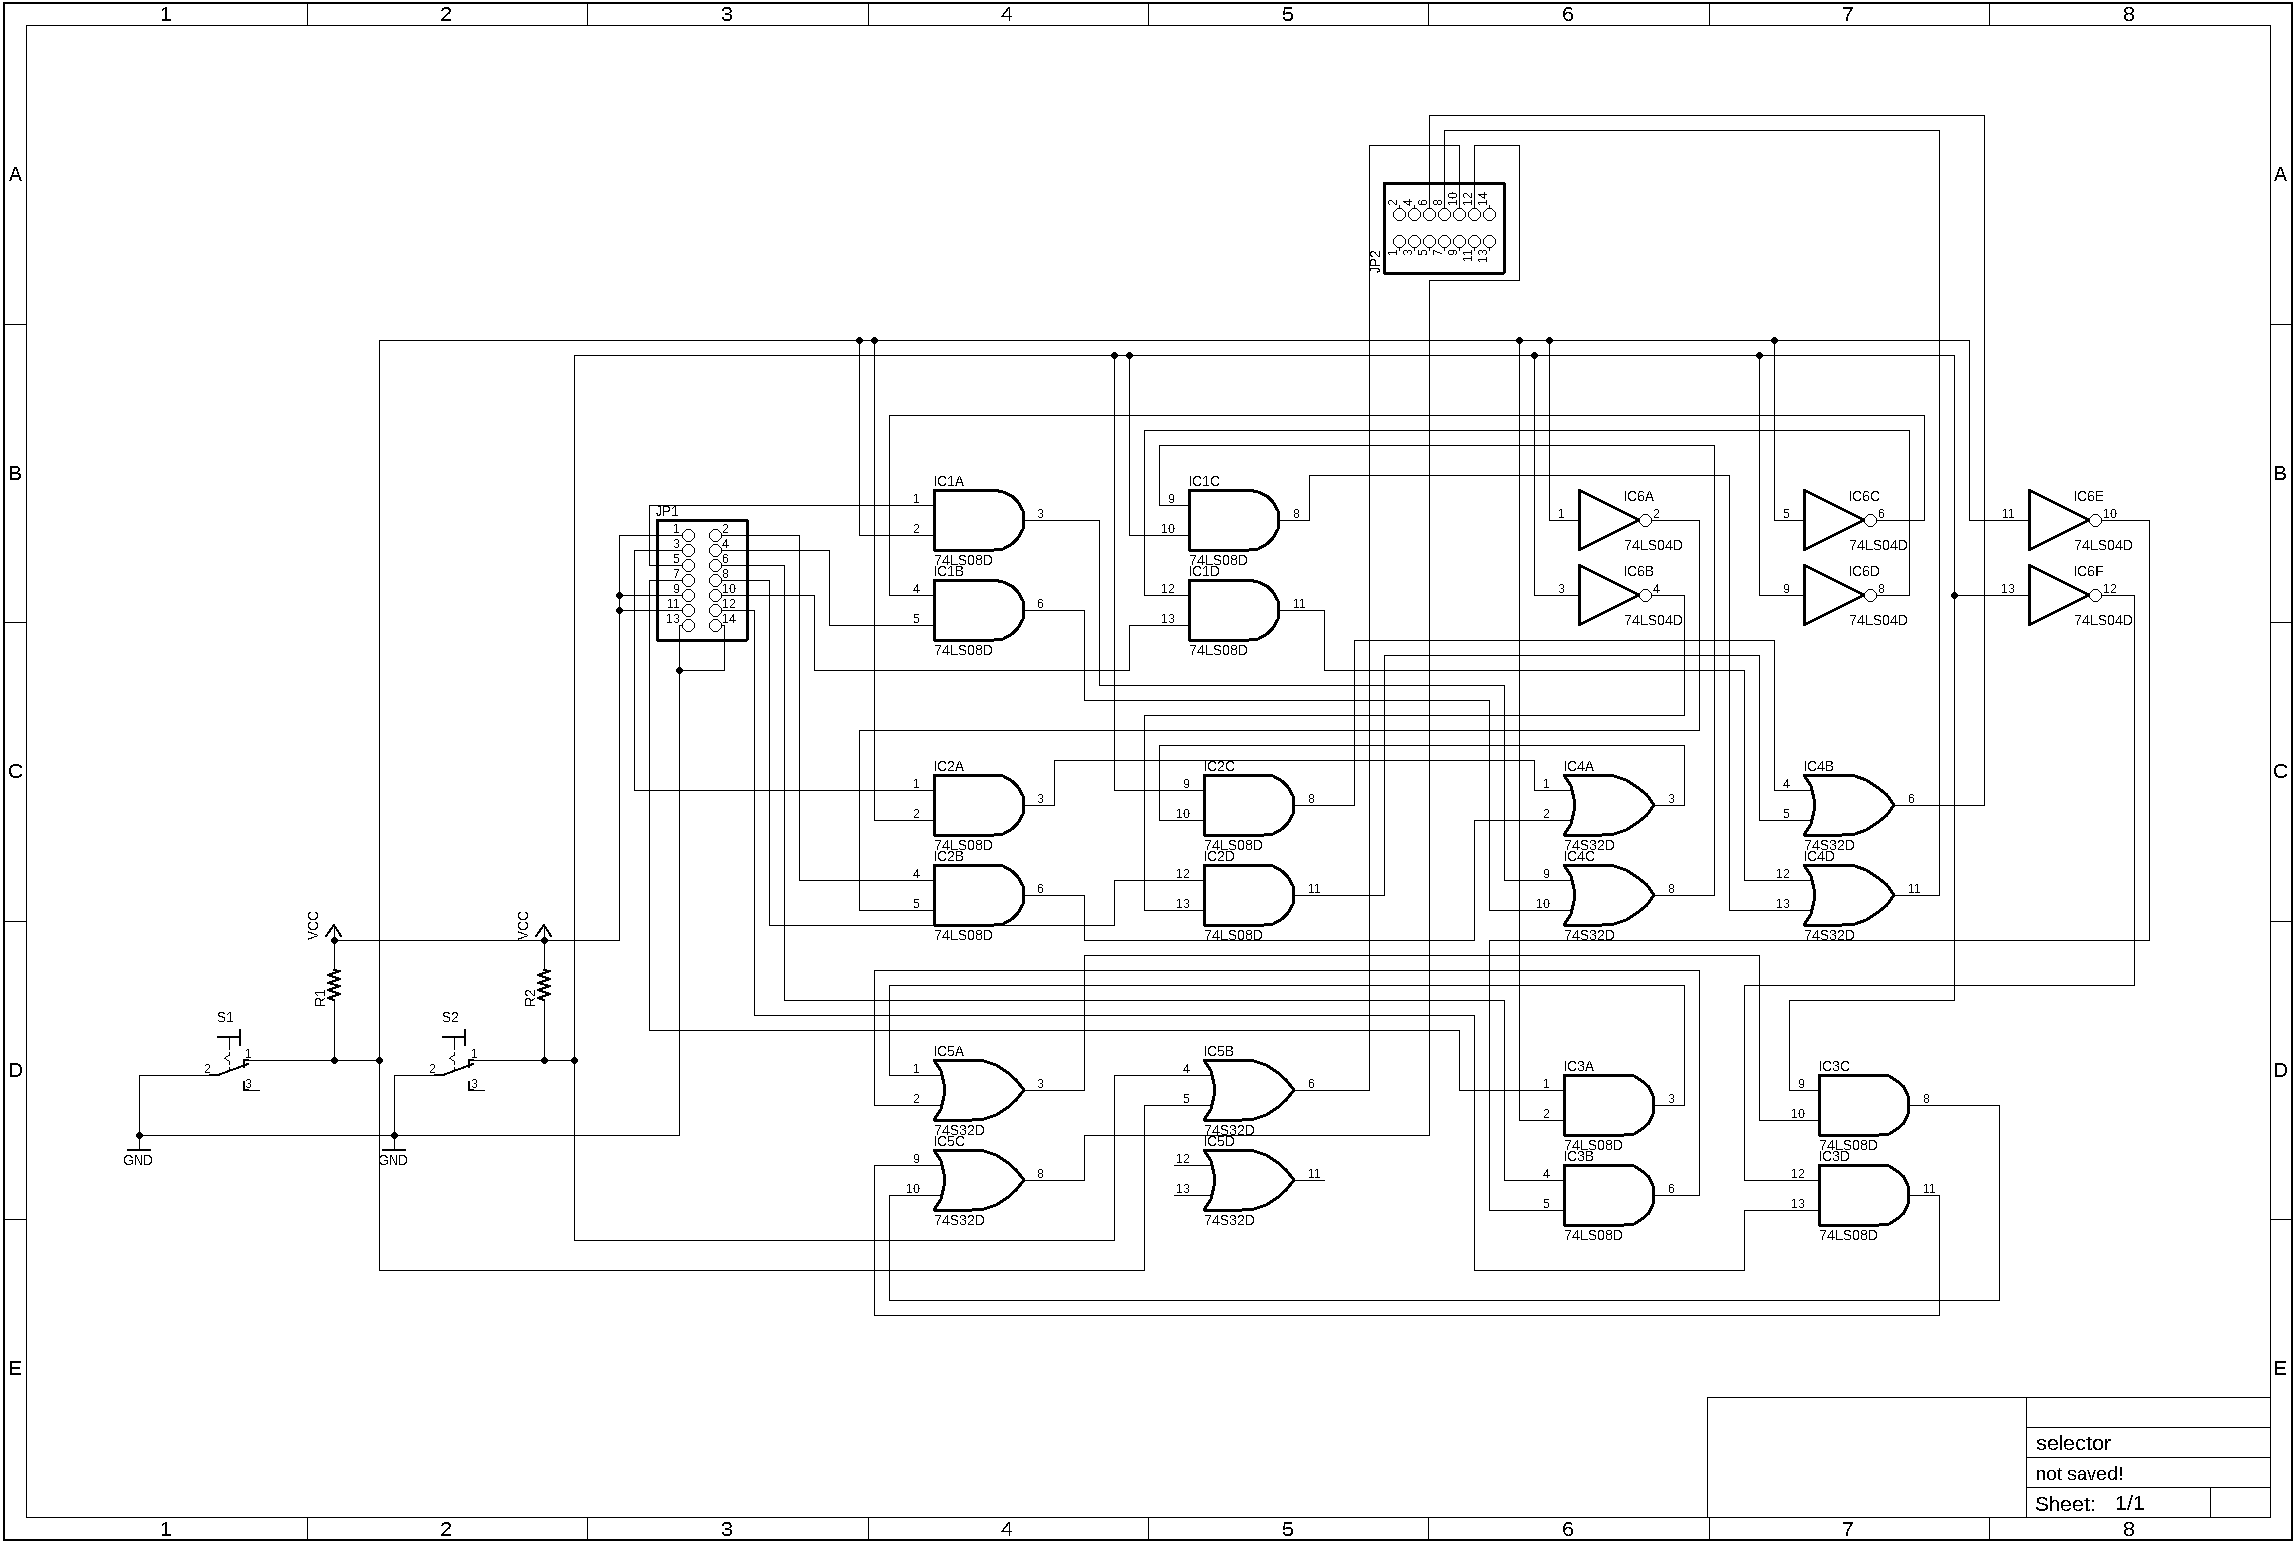
\includegraphics[angle = 90 , width =0.9\columnwidth]{./images/circuit.png}
  \caption{リバースエンジニアリングした回路図}
  \label{fig:reverse}
\end{figure}

\section{考察}
今回の実験では、セレクタ回路のリバースエンジニアリングを行った。リバースエンジニアリング
では、回路がどうなっているか予測しながら行うことで効率よく回路図を作成することが出来る
ことがわかった。

\end{document}